
%\section{Pattern Interface}


%Every pattern that runs on top of the framework should implement the Pattern\_I interface in order to be able to use the services provided by the framework. 
In order to make  certain ``plumbing'' functions easier, functions such as 
registering the pattern with the framework, bootstrapping the communication between the pattern and the framework (depending on the platform and type of deployment), we have defined a  \CPPClassName{PatternBase} helper class.
\CPPClassName{PatternBase} provides a member variable called FRAMEWORK which provides the functions available on the framework side and defines virtual functions that must be implemented by a Pattern, to handle the Events generated by framework. That is, the PatternBase class defines the shim layer for the Patterns and its implementation would vary from platform to platform. 

The chapter describes the \CPPClassName{PatternBase} class  and then explains how to drive from the \CPPClassName{PatternBase} class to implement a full-fledged Pattern use case.

\hypertarget{class_patterns_1_1_pattern_base}{}\section{Patterns\+:\+:Pattern\+Base Class Reference}
\label{class_patterns_1_1_pattern_base}\index{Patterns\+::\+Pattern\+Base@{Patterns\+::\+Pattern\+Base}}


Defines the abstract base class for patterns.  




{\ttfamily \#include $<$Pattern\+Base.\+h$>$}



Collaboration diagram for Patterns\+:\+:Pattern\+Base\+:
\nopagebreak
\begin{figure}[H]
\begin{center}
\leavevmode
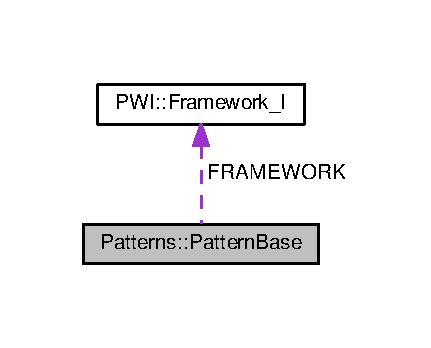
\includegraphics[width=207pt]{apis/class_patterns_1_1_pattern_base__coll__graph}
\end{center}
\end{figure}
\subsection*{Public Member Functions}
\begin{DoxyCompactItemize}
\item 
{\bfseries Pattern\+Base} (\hyperlink{namespace_core_1_1_naming_ab40d44ea919ec3e3c8cc05576ba6d610}{Pattern\+TypeE} type, char \+\_\+unique\+Name\mbox{[}128\mbox{]})\hypertarget{class_patterns_1_1_pattern_base_a994d3c33772d78e35ce2fac5f8913f33}{}\label{class_patterns_1_1_pattern_base_a994d3c33772d78e35ce2fac5f8913f33}

\item 
virtual bool \hyperlink{class_patterns_1_1_pattern_base_a4d36988129317f0e32de31ba0ed7982e}{Start} ()=0\hypertarget{class_patterns_1_1_pattern_base_a4d36988129317f0e32de31ba0ed7982e}{}\label{class_patterns_1_1_pattern_base_a4d36988129317f0e32de31ba0ed7982e}

\begin{DoxyCompactList}\small\item\em Starts the pattern, must be implemented by each pattern. \end{DoxyCompactList}\item 
virtual bool {\bfseries Stop} ()=0\hypertarget{class_patterns_1_1_pattern_base_a8bc96ad07ff84226659ed35f71619f89}{}\label{class_patterns_1_1_pattern_base_a8bc96ad07ff84226659ed35f71619f89}

\item 
virtual \hyperlink{class_patterns_1_1_pattern_base_a892f5cd6d58d75bb43e73cc38a3b882e}{$\sim$\+Pattern\+Base} ()\hypertarget{class_patterns_1_1_pattern_base_a892f5cd6d58d75bb43e73cc38a3b882e}{}\label{class_patterns_1_1_pattern_base_a892f5cd6d58d75bb43e73cc38a3b882e}

\begin{DoxyCompactList}\small\item\em Virtual destructor. \end{DoxyCompactList}\end{DoxyCompactItemize}
\subsection*{Public Attributes}
\begin{DoxyCompactItemize}
\item 
Recv\+Message\+Delegate\+\_\+t $\ast$ {\bfseries recv\+Delegate}\hypertarget{class_patterns_1_1_pattern_base_a51cc459a516bcf914b9ec91e198bc057}{}\label{class_patterns_1_1_pattern_base_a51cc459a516bcf914b9ec91e198bc057}

\item 
Neighbor\+Delegate $\ast$ {\bfseries nbr\+Delegate}\hypertarget{class_patterns_1_1_pattern_base_a62e4f5844c3b0573b5ef28696d5f4b36}{}\label{class_patterns_1_1_pattern_base_a62e4f5844c3b0573b5ef28696d5f4b36}

\item 
Dataflow\+Delegate\+\_\+t $\ast$ {\bfseries dataflow\+Delegate}\hypertarget{class_patterns_1_1_pattern_base_adbecd83eb5b30fb4df328d2b74949d30}{}\label{class_patterns_1_1_pattern_base_adbecd83eb5b30fb4df328d2b74949d30}

\item 
Control\+Response\+Delegate\+\_\+t $\ast$ {\bfseries control\+Delegate}\hypertarget{class_patterns_1_1_pattern_base_af563c486553ba15d62ea3fbb1bf7948b}{}\label{class_patterns_1_1_pattern_base_af563c486553ba15d62ea3fbb1bf7948b}

\end{DoxyCompactItemize}
\subsection*{Protected Member Functions}
\begin{DoxyCompactItemize}
\item 
virtual void {\bfseries Receive\+Message\+Event} (\hyperlink{class_core_1_1_message_t}{F\+Message\+\_\+t} \&msg)=0\hypertarget{class_patterns_1_1_pattern_base_a8adcc760cd5b3396971fcdcd5cd80bd4}{}\label{class_patterns_1_1_pattern_base_a8adcc760cd5b3396971fcdcd5cd80bd4}

\item 
virtual void {\bfseries Neighbor\+Update\+Event} (\hyperlink{struct_core_1_1_neighbor_update_param}{Neighbor\+Update\+Param} nbr\+Update)=0\hypertarget{class_patterns_1_1_pattern_base_acf80253c9df2790d99835dfb8c3c4544}{}\label{class_patterns_1_1_pattern_base_acf80253c9df2790d99835dfb8c3c4544}

\item 
virtual void {\bfseries Data\+Status\+Event} (\hyperlink{struct_core_1_1_dataflow_1_1_data_status_param}{Data\+Status\+Param} notification)=0\hypertarget{class_patterns_1_1_pattern_base_ae56e132583d61c4ca6df0dbcd761da09}{}\label{class_patterns_1_1_pattern_base_ae56e132583d61c4ca6df0dbcd761da09}

\item 
virtual void {\bfseries Control\+Response\+Event} (\hyperlink{struct_p_w_i_1_1_control_response_param}{Control\+Response\+Param} response)=0\hypertarget{class_patterns_1_1_pattern_base_a06b77e9f4bd2d16bad7afa8832642850}{}\label{class_patterns_1_1_pattern_base_a06b77e9f4bd2d16bad7afa8832642850}

\item 
void {\bfseries Register\+Pattern\+Delegates} (Pattern\+Id\+\_\+t pid, \hyperlink{namespace_core_1_1_naming_ab40d44ea919ec3e3c8cc05576ba6d610}{Pattern\+TypeE} \+\_\+type)\hypertarget{class_patterns_1_1_pattern_base_a9e619e83f88c871e62b3cea084b12d1a}{}\label{class_patterns_1_1_pattern_base_a9e619e83f88c871e62b3cea084b12d1a}

\item 
void {\bfseries Handle\+\_\+\+Register\+Response} (\hyperlink{struct_p_w_i_1_1_control_response_param}{Control\+Response\+Param} response)\hypertarget{class_patterns_1_1_pattern_base_aa834f9cdbc178916878211a6177701fe}{}\label{class_patterns_1_1_pattern_base_aa834f9cdbc178916878211a6177701fe}

\item 
void {\bfseries Random\+Local\+Spray} (Pattern\+Id\+\_\+t pid, \hyperlink{class_core_1_1_message_t}{F\+Message\+\_\+t} \&msg, Spray\+TypeE spraytype, bool israndomselection, \hyperlink{class_patterns_1_1_pattern_neighbor_table_i}{Patterns\+::\+Pattern\+Neighbor\+TableI} \&ptn\+Nbr\+Table, uint16\+\_\+t nonce)\hypertarget{class_patterns_1_1_pattern_base_ae17eb4a43493158ff5f146482041ca90}{}\label{class_patterns_1_1_pattern_base_ae17eb4a43493158ff5f146482041ca90}

\item 
bool {\bfseries Randomly\+Select\+Neighbor} (Neigbor\+Container\+Type \&selected\+Neighbor\+List, \hyperlink{class_patterns_1_1_pattern_neighbor_table_i}{Patterns\+::\+Pattern\+Neighbor\+TableI} \&ptn\+Nbr\+Table, Uniform\+Random\+Int $\ast$rand=N\+U\+LL)\hypertarget{class_patterns_1_1_pattern_base_af63159c86bda47a2492815735826dbab}{}\label{class_patterns_1_1_pattern_base_af63159c86bda47a2492815735826dbab}

\item 
void {\bfseries Send2\+Selected\+Neighbors} (Pattern\+Id\+\_\+t pid, Neigbor\+Container\+Type \&selected\+Neighbor\+List, \hyperlink{class_core_1_1_message_t}{F\+Message\+\_\+t} \&msg, uint16\+\_\+t nonce)\hypertarget{class_patterns_1_1_pattern_base_ac52dc18caa96893bd35d6c68970a5bec}{}\label{class_patterns_1_1_pattern_base_ac52dc18caa96893bd35d6c68970a5bec}

\end{DoxyCompactItemize}
\subsection*{Protected Attributes}
\begin{DoxyCompactItemize}
\item 
char {\bfseries unique\+Name} \mbox{[}128\mbox{]}\hypertarget{class_patterns_1_1_pattern_base_a6cff7cf408b665d720a0d2b82a0db9e8}{}\label{class_patterns_1_1_pattern_base_a6cff7cf408b665d720a0d2b82a0db9e8}

\item 
Pattern\+Id\+\_\+t {\bfseries P\+ID}\hypertarget{class_patterns_1_1_pattern_base_aa623ac5f4137e880067aff2092a8c732}{}\label{class_patterns_1_1_pattern_base_aa623ac5f4137e880067aff2092a8c732}

\item 
\hyperlink{class_p_w_i_1_1_framework___i}{Framework\+\_\+I} $\ast$ {\bfseries F\+R\+A\+M\+E\+W\+O\+RK}\hypertarget{class_patterns_1_1_pattern_base_a88b5eb77647f9e40ea741eaf6390d8bf}{}\label{class_patterns_1_1_pattern_base_a88b5eb77647f9e40ea741eaf6390d8bf}

\item 
bool {\bfseries registered}\hypertarget{class_patterns_1_1_pattern_base_a4305a51ad736ccc47242857352d4fa19}{}\label{class_patterns_1_1_pattern_base_a4305a51ad736ccc47242857352d4fa19}

\item 
Pattern\+Request\+StateE {\bfseries request\+State}\hypertarget{class_patterns_1_1_pattern_base_a93a8305be5ae2773af6e24fc18b5a689}{}\label{class_patterns_1_1_pattern_base_a93a8305be5ae2773af6e24fc18b5a689}

\item 
Pattern\+StateE {\bfseries pattern\+State}\hypertarget{class_patterns_1_1_pattern_base_aea5b5ffd6a1c809aa63fefe37ab79c1c}{}\label{class_patterns_1_1_pattern_base_aea5b5ffd6a1c809aa63fefe37ab79c1c}

\item 
uint32\+\_\+t {\bfseries n\+\_\+\+Expected\+Framework\+Responses}\hypertarget{class_patterns_1_1_pattern_base_a5898c2c8a20f9b949abe14cc85cea048}{}\label{class_patterns_1_1_pattern_base_a5898c2c8a20f9b949abe14cc85cea048}

\end{DoxyCompactItemize}


\subsection{Detailed Description}
Defines the abstract base class for patterns. 

The documentation for this class was generated from the following file\+:\begin{DoxyCompactItemize}
\item 
Tuscarora\+F\+W/\+Include/\+Interfaces/\+Pattern/Pattern\+Base.\+h\end{DoxyCompactItemize}
